\section{Introduction}
\label{sec:intro}

\begin{figure}[t]
    \centering
    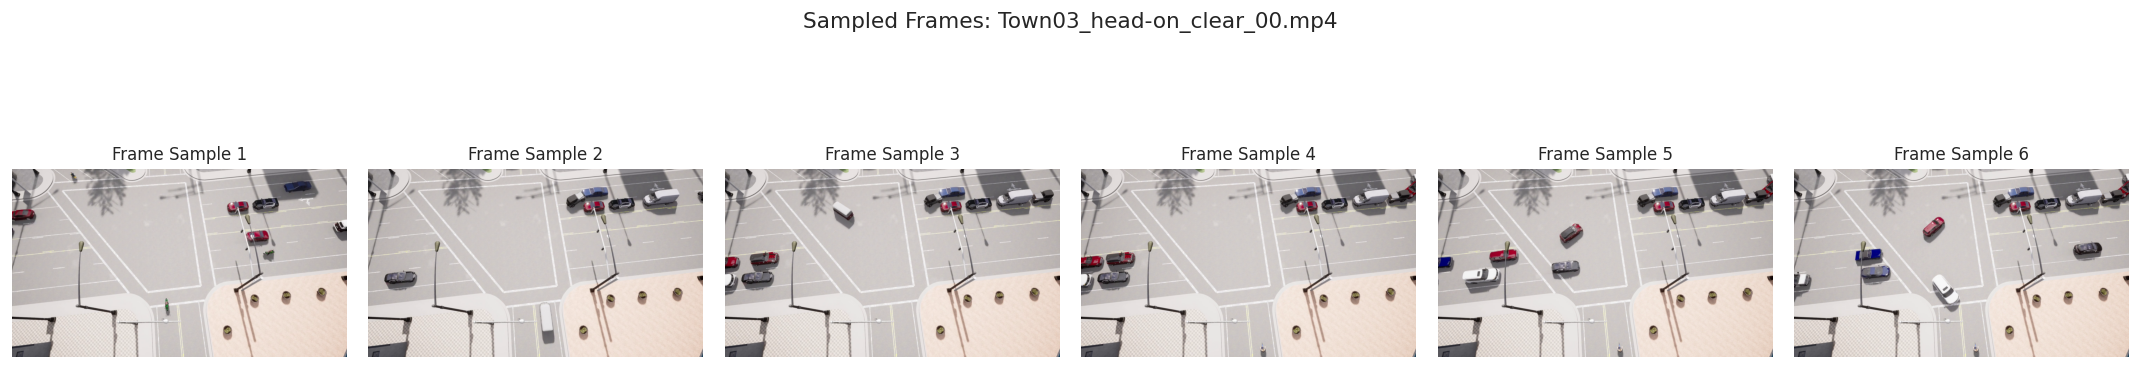
\includegraphics[width=\linewidth]{fig/sampled_frames.png}
    \caption{Chronological sampled frames from a synthetic CARLA traffic incident in the ACCIDENT @ CVPR 2026 dataset. Most clips record approximately 18 seconds of motion at 20 FPS resolution.}
    \label{fig:sampled_frames}
\end{figure}

Road traffic crashes kill over one million people each year according to the World Health Organization~\cite{who2023road}. Surveillance cameras installed at intersections and along highways record continuous footage that captures the circumstances of many of these incidents. If this footage could be analyzed automatically, emergency dispatchers would receive faster alerts and investigators would gain access to objective scene reconstructions. Yet most current detection methods require supervised training on annotated video from the same deployment environment~\cite{sultani2018real, yao2022dota}, which makes them expensive to transfer across camera installations with different viewpoints, lighting, and traffic patterns.

The ACCIDENT @ CVPR 2026 competition~\cite{accident2026} tests whether accident analysis can work without any labeled real-world data. Participants receive only synthetic videos generated by the CARLA simulator~\cite{dosovitskiy2017carla} for development (see Figure~\ref{fig:sampled_frames}); the test set is composed of real CCTV recordings and manual annotation of it is prohibited.

Three predictions are required per video: (1) the accident time in seconds, (2) normalized spatial coordinates of the impact point, and (3) the collision type from a five-class taxonomy (head-on, rear-end, sideswipe, single-vehicle, t-bone). Scoring uses the harmonic mean of a Gaussian temporal similarity, a Gaussian spatial similarity, and top-1 classification accuracy, so a poor prediction in any one dimension pulls the overall score down.

We address each target with a separate module. Temporal localization runs statistical anomaly detection on pixel-intensity differences between consecutive frames. Spatial localization accumulates dense optical flow magnitudes and extracts a weighted centroid. Collision classification passes frames near the detected peak through CLIP~\cite{radford2021learning}, a contrastive vision-language model trained on 400 million image-text pairs, and selects the class whose text prompts produce the highest cosine similarity. Because the modules are independent, any one of them can be swapped or tuned without modifying the rest. The full pipeline is implemented in a public Kaggle notebook~\cite{thakur2026notebook}.
